\chapter{Diseño e implementación} % Main chapter title

\label{Chapter3} % Change X to a consecutive number; for referencing this chapter elsewhere, use \ref{ChapterX}

En este capítulo se exponen los criterios de selección para la arquitectura de la plataforma de emulación. Se presenta la arquitectura elegida y se describe la estructura y organización de las capas de programación.


\definecolor{mygreen}{rgb}{0,0.6,0}
\definecolor{mygray}{rgb}{0.5,0.5,0.5}
\definecolor{mymauve}{rgb}{0.58,0,0.82}

%%%%%%%%%%%%%%%%%%%%%%%%%%%%%%%%%%%%%%%%%%%%%%%%%%%%%%%%%%%%%%%%%%%%%%%%%%%%%
% parámetros para configurar el formato del código en los entornos lstlisting
%%%%%%%%%%%%%%%%%%%%%%%%%%%%%%%%%%%%%%%%%%%%%%%%%%%%%%%%%%%%%%%%%%%%%%%%%%%%%
\lstset{ %
  backgroundcolor=\color{white},   % choose the background color; you must add \usepackage{color} or \usepackage{xcolor}
  basicstyle=\footnotesize,        % the size of the fonts that are used for the code
  breakatwhitespace=false,         % sets if automatic breaks should only happen at whitespace
  breaklines=true,                 % sets automatic line breaking
  captionpos=b,                    % sets the caption-position to bottom
  commentstyle=\color{mygreen},    % comment style
  deletekeywords={...},            % if you want to delete keywords from the given language
  %escapeinside={\%*}{*)},          % if you want to add LaTeX within your code
  %extendedchars=true,              % lets you use non-ASCII characters; for 8-bits encodings only, does not work with UTF-8
  %frame=single,	                % adds a frame around the code
  keepspaces=true,                 % keeps spaces in text, useful for keeping indentation of code (possibly needs columns=flexible)
  keywordstyle=\color{blue},       % keyword style
  language=[ANSI]C,                % the language of the code
  %otherkeywords={*,...},           % if you want to add more keywords to the set
  numbers=left,                    % where to put the line-numbers; possible values are (none, left, right)
  numbersep=5pt,                   % how far the line-numbers are from the code
  numberstyle=\tiny\color{mygray}, % the style that is used for the line-numbers
  rulecolor=\color{black},         % if not set, the frame-color may be changed on line-breaks within not-black text (e.g. comments (green here))
  showspaces=false,                % show spaces everywhere adding particular underscores; it overrides 'showstringspaces'
  showstringspaces=false,          % underline spaces within strings only
  showtabs=false,                  % show tabs within strings adding particular underscores
  stepnumber=1,                    % the step between two line-numbers. If it's 1, each line will be numbered
  stringstyle=\color{mymauve},     % string literal style
  tabsize=2,	                   % sets default tabsize to 2 spaces
  title=\lstname,                  % show the filename of files included with \lstinputlisting; also try caption instead of title
  morecomment=[s]{/*}{*/}
}


%----------------------------------------------------------------------------------------
%	SECTION 1
%----------------------------------------------------------------------------------------
\section{Introducción}
El principal criterio de selección de la arquitectura del emulador se fundamentó en el análisis de la arquitectura del sistema operativo \textit{mbed} y cómo funciona dentro de su simulador. La fase inicial de investigación permitió adquirir una comprensión del comportamiento de los perifericos simulados, las interacciones y las configuraciones necesarias para la plataforma web. 

Sin embargo, durante el análisis del repositorio, la presencia de múltiples módulos de código, bibliotecas y configuraciones que no estaban directamente relacionados con la simulación, inicialmente generó incertidumbre sobre su propósito y relevancia en la plataforma del simulador.
 
Después, al eliminar módulos y dependencias innecesarias, se procedió a evaluar la compatibilidad de su arquitectura. Durante el proceso, en primer lugar, se analizó si la arquitectura proporcionaba funcionalidades para la interacción con los usuarios. Incluso, de ser escalable y capaz de manejar nuevos desarrollos. 

Además, la mantenibilidad y flexibilidad también fueron aspectos evaluados. Otro punto esencial, fueron las tecnologías y herramientas utilizadas, lo cual implicó una curva de aprendizaje adicional. 

Asimismo, \textit{emscripten} fue fundamental para el desarrollo de la plataforma, y debido a la experiencia previa con el uso de cross-compiling toolchains para el kernel de Linux, facilitó la transición y ayudó en la comprensión de los conceptos y las herramientas relacionadas con \textit{emscripten}.

Finalmente, una vez confirmada su compatibilidad para los propósitos del presente trabajo, se tomó la decisión de seleccionarlo y empezar el desarrollo.
\hfill \break
\hfill \break
\hfill \break
\hfill \break

\section{Arquitectura de la plataforma web}



En el diagrama de bloques de la figura \ref{fig:Arquitectura} se muestra la arquitectura básica de una aplicación de usuario que ejecuta el emulador de la placa EDU-CIAA-NXP.


\begin{figure}[ht]
	\centering
	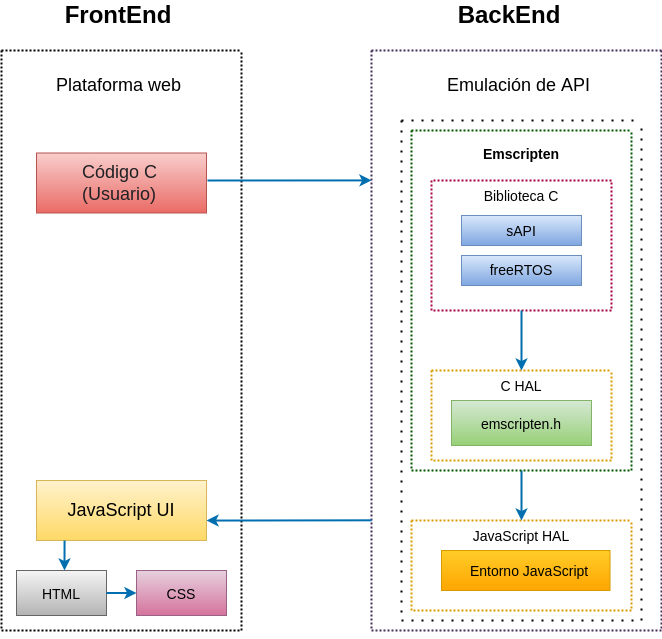
\includegraphics[scale=.55]{./Figures/Arquitectura.png}
	\caption{Diagrama de bloques arquitectura de la plataforma.}
	\label{fig:Arquitectura}
\end{figure}


La emulación a nivel de API proporciona una capa de abstracción para el entorno de desarrollo del usuario, de modo que permite escribir aplicaciones en \textit{C} y ejecutarlas en la plataforma de emulación. 

Al utilizar esta capa de abstracción, se pudo replicar las funcionalidades y las características de configuración de la biblioteca \textit{\textbf{sAPI}} del proyecto CIAA en un entorno diferente, en este caso, en un entorno web.

\hfill \break
\hfill \break
\hfill \break
\hfill \break
\hfill \break
\hfill \break
\hfill \break
\hfill \break
\hfill \break
\hfill \break




\section{Backend}

En esta capa de programación se desarrolló toda la lógica necesaria para emular las funcionalidades que proporcionan las bibliotecas: \textit{\textbf{sAPI}}, \textit{\textbf{freertos}} y \textit{\textbf{seos\textunderscore pont}} para la placa EDU-CIAA-NXP.

\subsection{Biblioteca C}

En primer lugar, se identificaron las funciones de las bibliotecas \textit{C} originales para empezar a emular. Luego, en el emulador se crearon interfaces que reflejen las estructuras de las bibliotecas originales, que incluyo definiciones de funciones, estructuras de datos y constantes.

Es decir, en las funciones originales se examinaron los parámetros de entrada y los valores de retorno, para luego mapearlos correctamente en las definiciones de las funciones del emulador.  A modo de referencia se muestra en la tabla \ref{tab:gpioMap} las definiciones de las funciones para \texttt{sapi\_gpio.h}, que incluye los nombres de la funciones, los tipos de parámetros y el tipo de valor de retorno. Cabe destacar que estas definiciones son idénticas tanto en las \textit{\textbf{sAPI}} como en el emulador, lo que permite una fácil correspondencia entre ambas.

\begin{table}[h]
	\centering
	\caption[Módulo \textit{GPIO}]{Módulo \textit{GPIO}}
	\begin{tabular}{l c c}    
		\toprule
		\textbf{Nombre de la función} 	 & \textbf{Parámetros} 		& \textbf{Tipo de retorno}  \\
		\midrule
		gpioInit & gpioMap\_t, gpioInit				&  bool\_t \\		
		gpioRead	 & gpioMap\_t				&  bool\_t \\
		gpioWrite	 & gpioMap\_t, bool\_t				&  bool\_t \\
		gpioToggle	 & gpioMap\_t				&  bool\_t \\
		\bottomrule
		\hline
	\end{tabular}
	\label{tab:gpioMap}
\end{table}



Al igual que en la biblioteca \textit{\textbf{sAPI}} del proyecto CIAA, los archivos de código fuente para la plataforma de emulación, conservan el mismo nombre, por ejemplo  \texttt{sapi\_gpio.c}. Sin embargo, la implementación de las funciones es totalmente distinta. En el caso de la biblioteca \textit{\textbf{sAPI}} del proyecto CIAA, para \texttt{sapi\_gpio.c}  se incluyen los archivos de encabezado: \texttt{gpio\_18xx\_43xx.h} y \newline \texttt{scu\_18xx\_43xx.h}. Y en el caso de la plataforma de emulación se usa otro archivos de encabezado como \texttt{gpio\_api.h} para replicar el mismo comportamiento.

A continuación, se presenta una comparación entre las clases del módulo gpio de la biblioteca \textit{\textbf{sAPI}} del proyecto CIAA y el módulo gpio implementado en la plataforma de emulación. 

La figura \ref{fig:GPIOsAPI} muestra las clases que se usan para la implementación de \newline \texttt{sapi\_gpio.c} del proyecto CIAA y en la figura \ref{fig:GPIOEmulador} se muestran otras clases para el mismo módulo.

\hfill \break
\hfill \break
\hfill \break
\hfill \break
\hfill \break
\hfill \break
\hfill \break
\hfill \break
\hfill \break
\hfill \break
\hfill \break
\hfill \break
\hfill \break

\begin{figure}[ht]
	\centering
	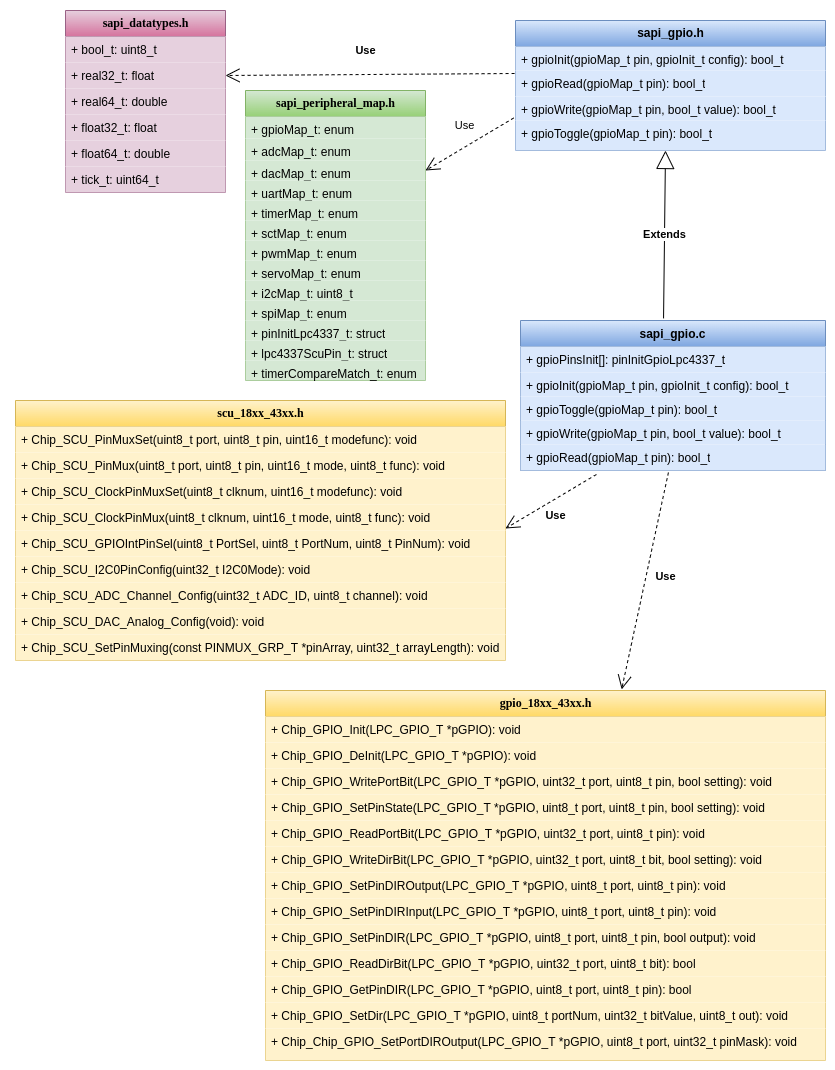
\includegraphics[scale=.41]{./Figures/DiagramaClasesGPIOsAPI.png}
	\caption{Diagrama de clases del módulo \textit{GPIO} de la biblioteca \textit{\textbf{sAPI}} del proyecto CIAA.}
	\label{fig:GPIOsAPI}
\end{figure}


\hfill \break
\hfill \break
\hfill \break
\hfill \break
\hfill \break
\hfill \break
\hfill \break

\begin{figure}[ht]
	\centering
	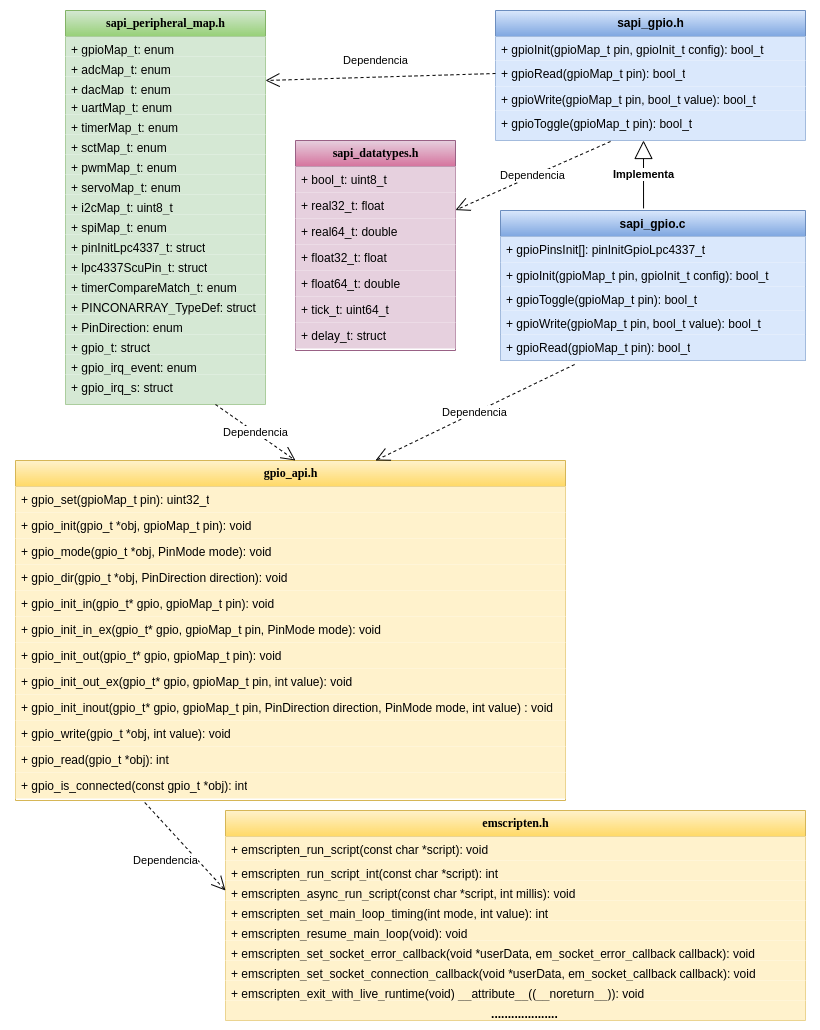
\includegraphics[scale=.41]{./Figures/DiagramaClasesEmulador.png}
	\caption{Diagrama de clases del módulo \textit{GPIO} de la plataforma de emulación para la placa EDU-CIAA-NXP.}
	\label{fig:GPIOEmulador}
\end{figure}


En ese sentido, para los demás archivos de la biblioteca \textit{C} de la plataforma de emulación, se siguió con la misma lógica. Asimismo, se utilizó un esquema de nomenclatura de los archivos de encabezado y de código fuente similar al de las bibliotecas originales.  Esto permitió mantener una estructura organizada y coherente en la emulación, que facilita el mantenimiento y comprensión.


También, se reservo el archivo de encabezado \texttt{sapi.h} que cumple con la misma funcionalidad que en la biblioteca \textit{\textbf{sAPI}} del proyecto CIAA, de tal forma que permita mediante su inclusión en la aplicación de usuario, usar todos los archivos que se necesitan.  

Además, se reutilizaron los archivos de encabezado: \texttt{sapi\_datatypes.h} y \newline \texttt{sapi\_peripheral\_map.h} incluidos en todos los módulos de la biblioteca \textit{\textbf{sAPI}} del proyecto CIAA. La decisión de reutilización fue para emular las características de hardware y prevalecer el uso de todos los tipos de datos básicos y configuraciones de la placa.

En la tabla \ref{tab:ConfiguracionGPIO} se muestran los tipos de datos de \texttt{sapi\_peripheral\_map.h} que se usan en la plataforma de emulación. De manera que, se puede observar que se reservan los nombres: TEC1, TEC2, TEC3 y TEC4 para los botones y los nombres LEDR, LEDG, LEDB, LED1, LED2 y LED3 para los LEDs de la placa EDU-CIAA-NXP.

\begin{table}[h]
	\centering
	\caption[\texttt{sapi\_peripheral\_map.h}.]{\texttt{sapi\_peripheral\_map.h}.}
	\begin{tabular}{l c c c}    
		\toprule
		\textbf{P2 header} & \textbf{P1 header} & \textbf{LEDs}  & \textbf{Switches}\\
		\midrule
		GPIO8, GPIO7, GPIO5 & T\_FIL1 &  LEDR &  TEC1\\		
		GPIO3, GPIO1, LCD1 & T\_COL2  & LEDG &  TEC2\\
		LCD2, LCD3, LCDRS & T\_COL0 & LEDB &  TEC3\\
		LCD4, SPI\_MISO, ENET\_TXD1 & T\_FIL2 & LED1 & TEC4\\
		ENET\_TXD0, ENET\_MDIO, ENET\_CRS\_DV & T\_FIL3 & LED2 & \\
	    ENET\_MDC, ENET\_TXEN, ENET\_RXD1 & T\_FIL0 & LED3 & \\
	    GPIO6, GPIO4, GPIO2 & T\_COL1&  & \\
	    GPIO0, LCDEN, SPI\_MOSI, ENET\_RXD0 & CAN\_TD&  & \\
		\bottomrule
		\hline
	\end{tabular}
	\label{tab:ConfiguracionGPIO}
\end{table}



\subsubsection{\textit{\textbf{sapi\_tick}}}

En la tabla \ref{tab:sapiTick} se puede observar las funciones del archivo de código fuente \texttt{sapi\_tick} en la biblioteca \textit{\textbf{sAPI}} del proyecto CIAA y en el emulador.

\begin{table}[h]
	\centering
	\caption[Funciones \texttt{sapi\_tick}]{Funciones \texttt{sapi\_tick}}
	\begin{tabular}{p{0.20\linewidth} p{0.50\linewidth}  p{0.20\linewidth}}    
		\toprule
		\textbf{Función} 	 & \textbf{Parámetros} 		& \textbf{Tipo de retorno}  \\
		\midrule
		tickInit & tick\_t tickRateMSvalue 		&  bool\_t \\		
		tickRead	 & void				&  tick\_t \\
		tickWrite	 & tick\_t ticks 				& void \\
		tickCallbackSet	 & callBackFuncPtr\_t tickCallback, void* tickCallbackParams				&  bool\_t \\
		tickPowerSet & bool\_t power 		&  void \\	
		\bottomrule
		\hline
	\end{tabular}
	\label{tab:sapiTick}
\end{table}

Para emular a nivel de API, se tuvo como objetivo replicar el comportamiento de la función \texttt{tickInit}, la cual se encarga de la inicialización y configuración de la interrupción del temporizador en la placa física. Sin embargo, al realizar la emulación en la plataforma web, esta función no se encuentra disponible de forma nativa. Por lo tanto, fue necesario emular su comportamiento y proporcionar una alternativa compatible.

Para lograr emular la funcionalidad de \texttt{SysTick\_Config}, se utilizó la capa de emulación correspondiente a \textit{C HAL}, que se ira detallando en las siguientes secciones. Esta capa de emulación permitió ejecutar código \textit{javaScript} en el contexto de \textit{emscripten}, lo que posibilitó replicar el comportamiento del temporizador \textit{SysTick}. 

Por otra parte, en la implementación de la \textit{\textbf{sAPI}} de la CIAA, el período se calcula multiplicando la frecuencia del reloj del sistema \texttt{SystemCoreClock} por \texttt{tickRateMSvalue} y dividiendo el resultado por 1000, Sin embargo, en el emulador, el período se corresponde directamente con el valor de \texttt{tickRateMSvalue}, lo que puede llevar a ciertas imprecisiones de tiempo.

En la siguiente tabla \ref{tab:ConfiguracionTicks} se muestran las diferencias en el enfoque de la implementación de la \textit{\textbf{sAPI}} de la CIAA y el emulador.

\begin{table}[h]
\centering
\caption[Comparación de la configuración de \textit{\textbf{sAPI}} de la CIAA y la Plataforma de Emulación.]{Comparación de la configuración de \textit{\textbf{sAPI}} de la CIAA y la Plataforma de Emulación.}
\begin{tabular}{p{0.15\linewidth} p{0.20\linewidth}  p{0.47\linewidth}}
\toprule
\textbf{Plataforma} 
& \textbf{Temporizador}
& \textbf{Frecuencia}
\\
\midrule
\textit{\textbf{sAPI}} CIAA & SysTick & \texttt{SystemCoreClock * tickRateMSvalue / 1000}  \\
Emulador &  Emscripten & \texttt{tickRateMSvalue} en milisegundos \\

\bottomrule
\hline
\end{tabular}
\label{tab:ConfiguracionTicks}
\end{table}

Una vez habilitada la interrupción del temporizador, se realiza una invocación periódica a la función \texttt{tickerCallback}, que tiene la misma implementación que en \texttt{sapi\_tick} de la biblioteca \textit{\textbf{sAPI}} del proyecto CIAA. La función \newline \texttt{tickerCallback} realiza las siguientes acciones: incrementa los contadores de ticks y, si el puntero \texttt{tickHookFunction} no es nulo, lo ejecuta pasando los parámetros \texttt{callBackFuncParams}. En consecuencia, esto permite la ejecución de tareas específicas programadas por el usuario en cada interrupción del temporizador periódico.

En el siguiente capítulo se detallarán las diferencias encontradas al realizar las pruebas entre la placa y el emulador utilizando estas funciones.

En el contexto de la emulación a nivel de API, para implementar las demás bibliotecas de las \textit{\textbf{sAPI}}, se siguió el mismo esquema utilizado en \texttt{sapi\_tick}. primeramente, se identificaron las funciones que requerían interacción con el hardware de la placa. Luego, en la capa \textit{C HAL} se implementaron funciones de emulación con emscripten para reflejar el comportamiento del hardware.

\subsubsection{\textit{\textbf{freertos}}}

Para emular la funcionalidad de las tareas de \textit{freeRTOS} en el contexto del emulador web, se implementó una solución utilizando la biblioteca de eventos de \textit{mbed}. Entonces, para las funciones \texttt{xTaskCreate} y \texttt{xTaskCreateStatic}, se programaron funciones periódicas utilizando las siguientes funciones de la biblioteca de eventos: 

 
 \begin{itemize}
	\item \texttt{int equeue\_create}:  crea una cola de eventos, configura e inicializa los recursos de plataforma necesarios, como semáforos y mutexes.
	
	\item \texttt{int equeue\_call\_every}:  se utiliza para crear un evento periódico en la cola de eventos equeue, programando llamadas repetidas a una función en intervalos regulares.
	
	\item \texttt{int equeue\_post}: permite publicar un evento en la cola de eventos equeue, estableciendo el tiempo y estableciendo el evento en la cola para su posterior procesamiento.
	
	\item \texttt{void equeue\_dispatch}: se encarga de despachar los eventos en la cola de eventos equeue de manera continua, verificando los tiempo y realizando acciones específicas según la configuración.

	\item \texttt{void equeue\_destroy}: permite liberar y limpiar todos los recursos asociados a una cola de eventos, libera los mutexes, semáforos y memoria asignada.
\end{itemize}

Estas funciones permiten ejecutar tareas periódicas en intervalos de tiempo regulares, lo que proporcionó una aproximación simplificada para emular la funcionalidad de tareas en el emulador web. Aunque esta solución no ofrece todas las características de un sistema operativo de tiempo real completo como \textit{freeRTOS}, fue adecuada para simular el funcionamiento de programas de usuario simples.

Es importante destacar que la implementación de tareas en el emulador web tiene una limitación significativa. Debido a que solo puede ejecutar un subproceso (hilo de ejecución) a la vez, no es posible que se ejecuten tareas simultáneas. Esto significa que, a diferencia del sistema operativo de tiempo real \textit{freeRTOS}, donde se pueden crear múltiples tareas que se ejecutan de manera concurrente, en el emulador web solo es posible ejecutar una sola tarea. Por lo tanto, esta solución es adecuada para programas de usuario simples que no requieran multitarea.


La tabla \ref{tab:ConceptosRTOS} expone algunos de los conceptos importantes de \textit{freeRTOS} que se cumplen en el emulador.

\begin{table}[h]
\centering
\caption[Conceptos importantes de \textit{freeRTOS} que se cumplen en el emulador.]{Conceptos importantes de \textit{freeRTOS} que se cumplen en el emulador.}
\begin{tabular}{p{0.45\linewidth} p{0.15\linewidth}  p{0.15\linewidth}}
\toprule
\textbf{Capacidades} 
& \textbf{\textit{freeRTOS}}
& \textbf{Emulador}
\\
\midrule
Multitareas & Si & No  \\
Funciones de espera &  Si & Si \\
Cambio de contexto &  Si & Si \\
Tarea de procesamiento continuo &  Si & Si \\
Manejo de prioridades & Si & No  \\
\bottomrule
\hline
\end{tabular}
\label{tab:ConceptosRTOS}
\end{table}

En el emulador, se encuentran implementados varios conceptos importantes de \textit{freeRTOS}, como funciones de espera y cambio de contexto. Sin embargo, en esta primera versión del emulador, no se han incluido el manejo de multitareas y de prioridades presentes en \textit{freeRTOS}.


\subsubsection{\textit{\textbf{sapi\_delay}}}

La tabla \ref{tab:sapiDelay} expone las funciones del archivo de código fuente \texttt{sapi\_delay} en la biblioteca \textit{\textbf{sAPI}} del proyecto CIAA y en el emulador.

\begin{table}[h]
	\centering
	\caption[Funciones \texttt{sapi\_delay}]{Funciones \texttt{sapi\_delay}}
	\begin{tabular}{p{0.20\linewidth} p{0.50\linewidth}  p{0.20\linewidth}}    
		\toprule
		\textbf{Función} 	 & \textbf{Parámetros} 		& \textbf{Tipo de retorno}  \\
		\midrule
		delayInaccurateMs & tick\_t delay\_ms 		&  void \\		
		delayInaccurateUs	 & tick\_t delay\_us			&  void \\
		delayInaccurateNs	 & tick\_t delay\_ns				& void \\
		delay	 & tick\_t duration\_ms				&  void \\
		delayInit & delay\_t * delay, tick\_t duration 		&  void \\
		delayRead & delay\_t * delay 		&  bool\_t \\
		delayWrite & delay\_t * delay, tick\_t duration 		&  void \\	
		\bottomrule
		\hline
	\end{tabular}
	\label{tab:sapiDelay}
\end{table}

La función \texttt{delay} en la biblioteca \textit{\textbf{sAPI}} del proyecto CIAA crea una pausa en la ejecución del programa durante el tiempo especificado en \texttt{duration\_ms} implementando un bucle de espera. Este bucle se ejecutará mientras la diferencia de tiempo entre \texttt{tickRead()} y startTime(inicio actual de \texttt{tickRead()} sea menor que \texttt{duration\_ms/ tickRateMS}.

Sin embargo, cuando \textit{emscripten} compila código \textit{C} a \textit{javaScript}, la función \texttt{delay} tal como está escrita, causa que la ejecución de la plataforma web se bloquee o congele. Esto se debe a que la función \texttt{tickRead()} no se actualiza a la velocidad que se espera, lo que lleva a que se obtenga el mismo valor repetidamente. Es decir, debido a la naturaleza asincrónica de \textit{javaScript} y al no tener una pausa controlada en el bucle (como \texttt{delay(1)}), \textit{javaScript} no tiene tiempo suficiente para actualizar el valor de \texttt{tickRead()} entre iteraciones. De esta manera,  el bucle \texttt{while} se queda esperando activamente e impide al navegador atender otros eventos.

Por esta razón, se decidio usar en las funciones de espera,  las funciones nativas de \textit{emscripten} usando la capa de emulación \textit{C HAL}, que se ira detallando en la siguiente sección. En consecuencia, se aprovecho su eficiencia y precisión.


\subsection{C HAL}

La capa de Abstracción de Hardware en \textit{C (C HAL)}  permitió replicar el comportamiento del hardware de la placa, lo que a su vez posibilitó la compatibilidad de las bibliotecas de nivel superior escritas en \textit{C} en el entorno de emulación de la plataforma web.

En esta capa se encuentra la biblioteca \textit{emscripten.h}, la cual provee las funciones y macros necesarias para interactuar con el compilador de \textit{emscripten}. El compilador transforma el código \textit{C} a \textit{javaScript}, de esta manera, se facilita la interacción y comunicación entre el código \textit{C} y el entorno web, donde se ejecuta el código ya convertido a \textit{javaScript}.

\textit{Emscripten}, usa el compilador \textit{LLVM} que actualmente tiene la mayor compatibilidad con \textit{webAssembly}, y lo bueno de \textit{LLVM} es que el rendimiento del código generado es muy eficiente. 

Además, \textit{LLVM} proporciona múltiples componentes que pueden intercambiarse entre sí, a diferencia de los compiladores \textit{GCC} que presentan una estructura monolítica. Por tanto, \textit{emscripten} compila el código \textit{C} en un módulo \textit{webAssembly} para que luego permita ser ejecutado en la web.

En la figura \ref{fig:Emscripten} se muestra el diagrama con el principal funcionamiento de \textit{emscripten}. 
\hfill \break

\begin{figure}[ht]
	\centering
	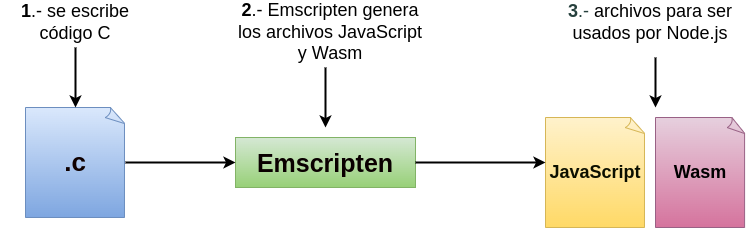
\includegraphics[scale=.50]{./Figures/Emscripten.png}
	\caption{Diagrama de funcionamiento de \textit{emscripten}.}
	\label{fig:Emscripten}
\end{figure}



Se puede observar que son dos los archivos generados:
\begin{itemize}
	\item Archivo \textit{JavaScript}.
	\item Archivo \textit{Wasm}.
\end{itemize}
El segundo es el archivo \textit{webAssembly} que contiene el código compilado, y el primero es un archivo \textit{javaScript} que contiene el soporte en tiempo de ejecución por \textit{NodeJS} para cargarlo y ejecutarlo.


En ese sentido, para la aplicación de usuario dentro de la plataforma, cuando se ejecuta un programa, por ejemplo blinky, \textit{emscripten} creará los archivos \textit{blinky.js}, \textit{blinky.wasm}, y adicionalmente creará otros archivos de configuración que son complementarios, los cuales son:

\begin{itemize}
	\item Archivo \textit{blinky.js.components}.
	\item Archivo \textit{blinky.wasm.map}.
	\item Archivo \textit{blinky.wast}.
\end{itemize}



\subsubsection{\textit{\textbf{sapi\_tick}}}

Para emular el comportamiento de la interrupción del temporizador \textit{SysTick} y proporcionar la invocación periódica a la función \texttt{tickerCallback} de \textit{sapi\_tick}, se utilizó la macro \texttt{EMSCRIPTEN\_KEEPALIVE} de \textit{emscripten}, que le dice al compilador de \textit{emscripten} que conserve la función marcada con esta macro en el código compilado, incluso si no es accedida desde el código \textit{javaScript} del lado del cliente.

Es decir, cuando la función marcada con la macro \texttt{EMSCRIPTEN\_KEEPALIVE} sea invocada desde la capa \textit{JavaScript HAL}, llamará a la función \texttt{tickerCallback} de la biblioteca \textit{C} y la ejecutará. En la figura \ref{fig:tickerCallback} se muestra el funcionamiento de \texttt{EMSCRIPTEN\_KEEPALIVE}. 


\begin{figure}[ht]
	\centering
	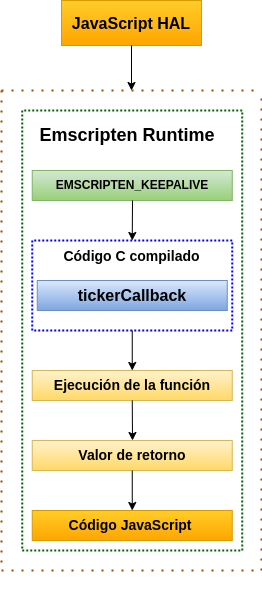
\includegraphics[scale=.42]{./Figures/tickerCallback.png}
	\caption{Diagrama de bloques \texttt{EMSCRIPTEN\_KEEPALIVE}.}
	\label{fig:tickerCallback}
\end{figure}


\subsubsection{\textit{\textbf{sapi\_delay}}}

Para emular las funciones de espera de la biblioteca \textit{C} se implemento la función \texttt{emscripten\_sleep}, que utiliza funciones asincrónicas internas de emscripten para realizar pausas. 

Por lo tanto, permite al navegador atender otros eventos mientras el programa se encuentra en espera. Es decir, evita el bloqueo de la ejecución del resto del código y también, que la página no responda.

Además, proporciona pausas precisas, debido a que, \textit{emscripten}  utiliza las capacidades de temporización del navegador para garantizar que el tiempo indicado sea realizado.

La figura \ref{fig:emscriptenDelay} representa el funcionamiento de  \texttt{emscripten\_sleep}. 

\begin{figure}[ht]
	\centering
	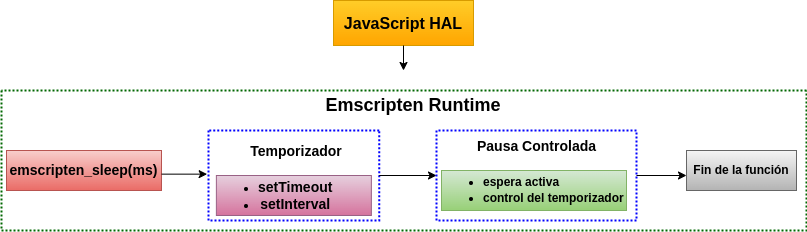
\includegraphics[scale=.53]{./Figures/emscriptenDelay.png}
	\caption{Diagrama de bloques \texttt{emscripten\_sleep.}}
	\label{fig:emscriptenDelay}
\end{figure}

\subsection{JavaScript HAL}

Esta capa de programación se diseñó para proporcionar la funcionalidad de distribuir los eventos entre los componentes de la interfaz de usuario de \textit{javaScript} y la capa \textit{C HAL}. Para lograr este objetivo se usaron las clases \textit{EventEmitter} del módulo \textit{Events} que monitorizan y activan los eventos. Además, facilita la interacción del navegador con el código \textit{javaScript} y la actualización de la interfaz de usuario de manera flexible y eficiente.

También, la clase \textit{EventEmitter} se basa en el modelo de publicación/suscripción que se trata de un paradigma de envío de mensajes asíncrono mediante el cual un usuario publica mensajes y uno o varios objetos se suscriben a esos eventos.

En la figura \ref{fig:PublicarSuscribir} se muestra el modelo de \textit{publicación/suscripción}.

\begin{figure}[ht]
	\centering
	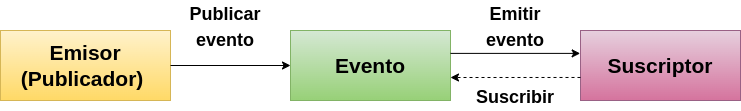
\includegraphics[scale=.49]{./Figures/PublicarSuscribir.png}
	\caption{Modelo de \textit{publicación/suscripción}.}
	\label{fig:PublicarSuscribir}
\end{figure}


Para la implementacion de esta capa de emulación, se crearon archivos \textit{javaScript} con instancias de la clase \textit{EventEmitter}, que al utilizar el método \textit{emit} lanzan eventos con nombre. El nombre del evento es un string y permite que los oyentes registrados al evento sean notificados. La figura \ref{fig:EventemitterNodejs} muestra el diagrama de bloques de la instancia de \textit{EventEmitter} en la plataforma de emulación.

\begin{figure}[ht]
	\centering
	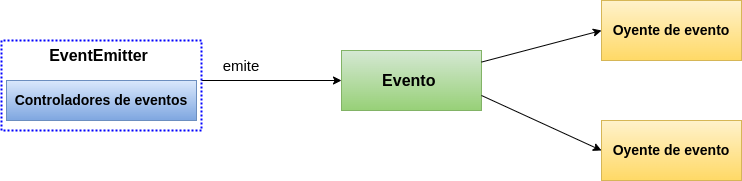
\includegraphics[scale=.49]{./Figures/EventemitterNodejs.png}
	\caption{Diagrama de bloques de \textit{EventEmitter} implementado en la plataforma.}
	\label{fig:EventemitterNodejs}
\end{figure}

En la sección de \textit{Caso de Estudio}, se mostrará la implementación de este modelo en los archivos \textit{javaScript} del emulador web.

\subsubsection{\textit{\textbf{sapi\_tick}}}

Para lograr la interacción con la capa de emulación \textit{C HAL}, y realizar la invocación periódica a la función que usa la macro \texttt{EMSCRIPTEN\_KEEPALIVE} de \textit{emscripten} se configuró en esta capa de desarrollo un temporizador de \textit{javaScript}.

Además, dentro del temporizador, se utilizó la función \texttt{ccall} de \textit{emscripten}, que permite invocar a la funcion \texttt{tickerCallback} desde el código \textit{C} compilado con \textit{emscripten}. 


A continuacion, se muestra en la figura  \ref{fig:ccall} el funcionamiento de \texttt{ccall}. 
\hfill \break
\hfill \break

\begin{figure}[ht]
	\centering
	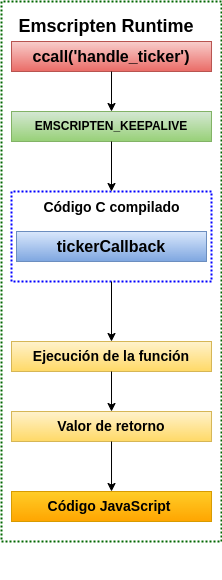
\includegraphics[scale=.49]{./Figures/ccall.png}
	\caption{Diagrama de bloques de la función \textit{ccall}.}
	\label{fig:ccall}
\end{figure}

Sin embargo, debido a la naturaleza asíncrona de \textit{javaScript} y al uso de la función \texttt{ccall}, la función no mantiene el contexto entre las ejecuciones del temporizador. En consecuencia, cada vez que se reinicia el temporizador y se ejecuta la función  \texttt{tickerCallback}, la tarea específica programada por el usuario comienza desde el principio en lugar de continuar desde el punto donde quedó anteriormente. 


\section{Frontend}
En esta parte de la plataforma web se implementó el desarrollo de la interacción entre el \textit{backend} y el navegador del usuario.


\subsection{JavaScript UI}

Esta capa se desarrolló con el propósito de que se comunique con la capa \textit{JavaScript HAL}, y también con el objetivo de proporcionar componentes de código, utilidades y manejo de eventos en la aplicación de usuario.

Por tanto, para lograr la comunicación con la capa \textit{JavaScript HAL}, se desarrolló en esta capa los objetos que se sucriben al detector de eventos programados en la \textit{HAL}.

\textit{JavaScript} permite crear oyentes, utilizando el método \texttt{on()} y pasando como argumento el nombre del evento al que se quiere suscribir. De esta manera, se  programaron varios subscriptores para un mismo evento en diferentes archivos \textit{javaScript} dentro de esta capa. En consecuencia, se logró una mayor interactividad entre los componentes de la plataforma.

Es decir, cuando se emite algún evento en la \textit{HAL}, entonces el oyente suscrito a ese evento en esta capa \textit{UI} lo podrá escuchar y realizar las acciones que correspondan para la funcionalidad requerida. La figura \ref{fig:EventemitterNodeJSUI} describe esta situación.


\begin{figure}[ht]
	\centering
	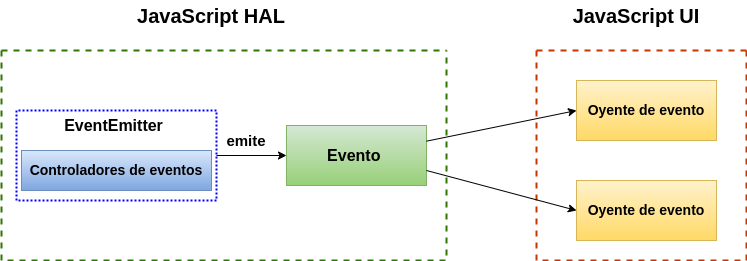
\includegraphics[scale=.51]{./Figures/EventemitterNodeJSUI.png}
	\caption{Diagrama de bloques de los oyentes de \textit{EventEmitter} en la capa UI.}
	\label{fig:EventemitterNodeJSUI}
\end{figure}




\subsection{Aplicación de Usuario}
La plataforma de emulación para la placa EDU-CIAA-NXP es una versión en línea, que se ejecuta en el \textit{browser} del usuario. Además, la interfaz fue diseñada como una herramienta que permite al usuario realizar sus tareas de programación dentro de una plataforma simple e intuitiva.

Sin embargo, existen algunas limitaciones que se deben tener en cuenta.

\begin{itemize}
	\item Las unidades de tiempo especificadas por los valores en las constantes, por ejemplo: 
	
\texttt{\#define TASK1\_PERIODICITY 1000} 

Cuando el usuario define \texttt{TASK1\_PERIODICITY} con un valor de 1000 para ser usado dentro del siguiente codigo:

\texttt{if( task1Counter++ == TASK1\_PERIODICITY )\{\newline} 
\texttt{  task1();}{\newline} 
\texttt{  task1Counter = 0;}{\newline} 
\texttt{\}}

Significa que la tarea  planificada se ejecutará cada 1000 milisegundos en la placa fisica. Sin embargo, en el emulador web, la velocidad de ejecución puede variar y no necesariamente coincidir con el tiempo real. Por lo tanto, el tiempo de ejecución de cada iteración de la tarea \texttt{task1} podría ser más lento en el emulador web, por ejemplo, 1000 segundos. Estas diferencias en la ejecución se deben a las limitaciones inherentes de \textit{javaScript} y \textit{emscripten}, que pueden afectar la precisión del tiempo.


	\item En el emulador dentro de un bucle infinito \texttt{while(1)}, es necesario agregar un retraso (\texttt{delay)}, de lo contrario, el navegador no puede actualizar la interfaz de la plataforma web ni responder a eventos del usuario. Esto significa que el navegador no tiene la oportunidad de realizar otras tareas o responder a eventos mientras el bucle está en ejecución. Como resultado, el navegador se bloquea o congela y puede dejar de responder.
	
\end{itemize}


\section{Caso de estudio}

Cuando un usuario ejecuta una aplicación simple como \textit{Blinky} que enciende un led, entonces, la plataforma reflejará la acción en su interfaz, permitiendo al usuario ver el resultado dentro del entorno virtual.


La figura \ref{fig:DiagramaSecuencia} muestra la interacción del usuario con los objetos del sistema y el orden en que se producen. Además, se muestra los mensajes que se pasan entre los objetos.


\begin{figure}[ht]
	\centering
	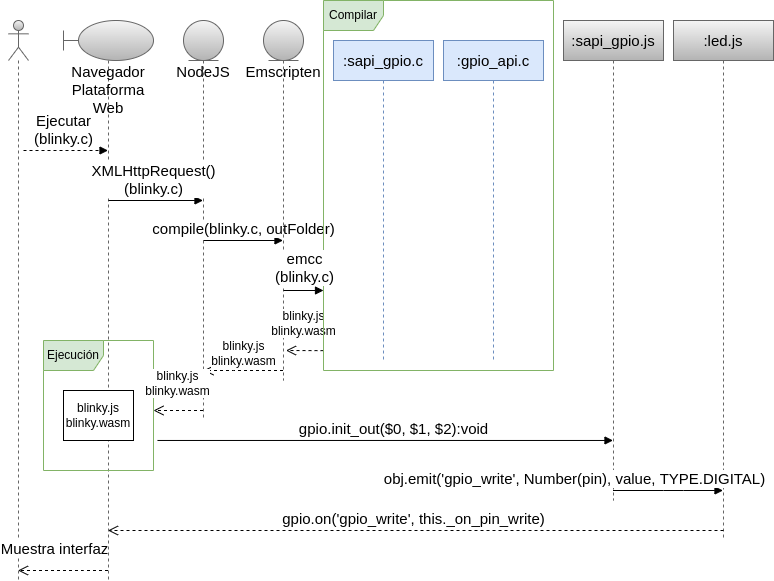
\includegraphics[scale=.49]{./Figures/DiagramaSecuencia.png}
	\caption{Interacción del usuario con los objetos del emulador.}
	\label{fig:DiagramaSecuencia}
\end{figure}


En la plataforma se crea un objeto nativo del navegador web \texttt{XMLHttpRequest} que permite hacer solicitudes HTTP desde JavaScript. Luego, en el servicio de \textit{backend} se invoca a la biblioteca \textit{C} \texttt{sapi\_gpio.c}, que llama a \texttt{gpio\_api.c} y mediante el uso de funciones nativas de \textit{emscripten} pasa el evento a la capa \textit{JavaScript HAL}. 

Además, mediante la función \textit{write} se realiza la activación del evento, por lo tanto, el objeto emitirá el evento con el nombre \texttt{gpio\_write} pasando como argumentos el número de pin, el valor dígital y el tipo de pin declarado. 

\hfill \break
\hfill \break
\hfill \break

La figura \ref{fig:GPIOEventEmitter} muestra el diagrama en bloques del evento con el nombre \newline \texttt{gpio\_write}.

\begin{figure}[ht]
	\centering
	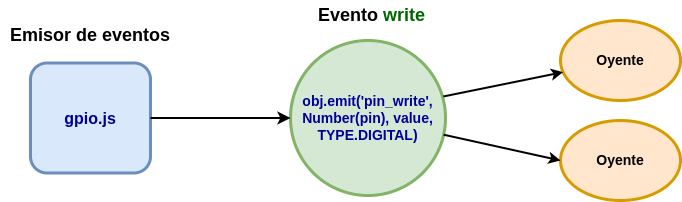
\includegraphics[scale=.50]{./Figures/GPIOEventEmitter.png}
	\caption{Activación de evento con el nombre \texttt{gpio\_write}.}
	\label{fig:GPIOEventEmitter}
\end{figure}



En ese sentido, en la capa \textit{JavaScript UI}  cuando se emite el evento con el nombre \texttt{gpio\_write}, entonces el oyente subscrito a ese evento lo podrá escuchar y realizar las acciones que corresponden para la funcionalidad que se pide.

La figura \ref{fig:ListeningGPIOEventEmitter} muestra el diagrama en bloques del oyente subscrito al evento \texttt{gpio\_write}.

\hfill \break

\begin{figure}[ht]
	\centering
	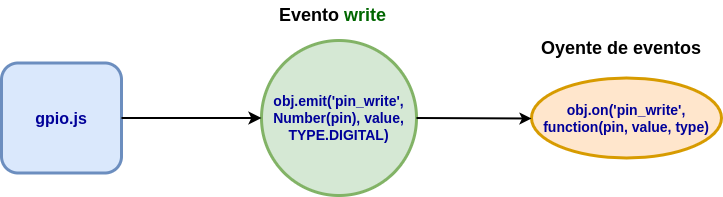
\includegraphics[scale=.50]{./Figures/ListeningGPIOEventEmitter.png}
	\caption{GPIO oyente del evento con el nombre \texttt{gpio\_write}.}
	\label{fig:ListeningGPIOEventEmitter}
\end{figure}

Entonces, en la plataforma web se muestrarán los cambios de \texttt{gpio\_write} en la placa virtual. 

En la figura \ref{fig:AplicacionUsuarioLeds} se presenta para una función de la GPIO, la interacción entre todas las capas de programación.

\hfill \break
\hfill \break
\hfill \break
\hfill \break
\hfill \break
\hfill \break
\hfill \break
\hfill \break
\hfill \break

\begin{figure}[ht]
	\centering
	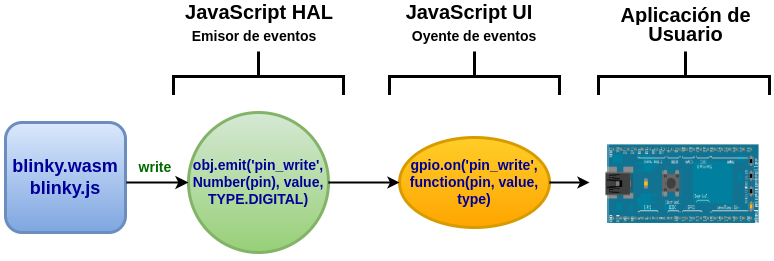
\includegraphics[scale=.40]{./Figures/AplicacionUsuarioLeds.png}
	\caption{Interacción entre todas las capas de programación.}
	\label{fig:AplicacionUsuarioLeds}
\end{figure}

\section{Diseño de la Interfaz de Usuario}

Para el desarrollo de la interfaz, se optó por un diseño intuitivo, de manera que el usuario se sienta familiarizado con las herramientas de trabajo y que la disposición de los componentes sea cómoda y esté organizada al momento de usarlas.

La figura \ref{fig:PlataformaEmulador1} muestra la parte izquierda de la interfaz gráfica para la aplicación de usuario 
y en la figura \ref{fig:PlataformaEmulador2} muestra la parte derecha de la interfaz gráfica para la aplicación de usuario.

\hfill \break
\hfill \break
\hfill \break
\hfill \break
\hfill \break
\hfill \break

\begin{figure}[ht]
	\centering
	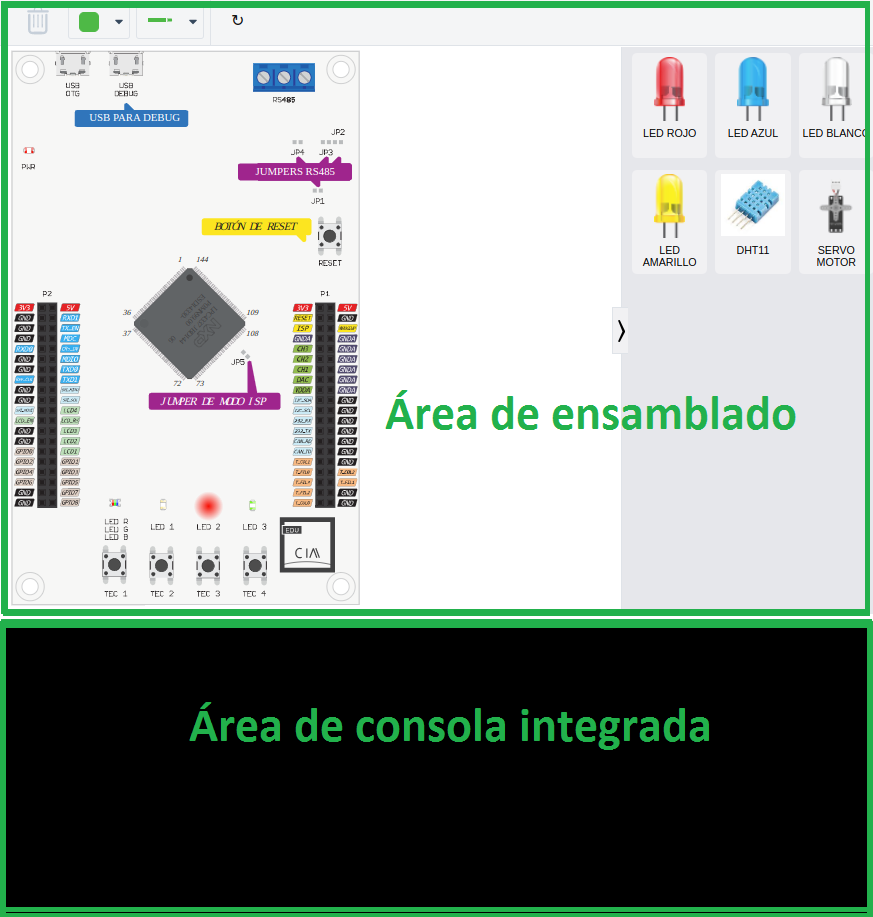
\includegraphics[scale=.60]{./Figures/PlataformaEmulador1.png}
	\caption{Parte izquierda de la plataforma de emulación para la placa EDU-CIAA-NXP.}
	\label{fig:PlataformaEmulador1}
\end{figure}

\hfill \break
\hfill \break
\hfill \break
\hfill \break
\hfill \break
\hfill \break
\hfill \break
\hfill \break
\hfill \break
\hfill \break
\hfill \break
\hfill \break
\hfill \break
\hfill \break
\hfill \break

\begin{figure}[ht]
	\centering
	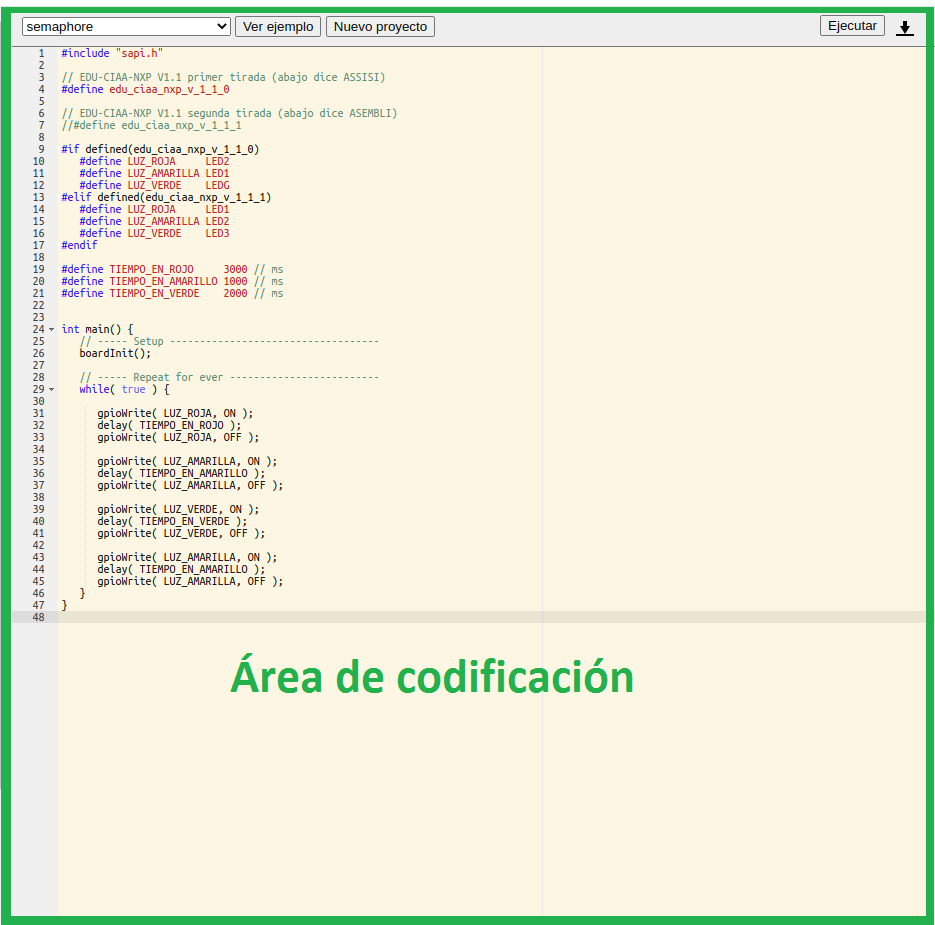
\includegraphics[scale=.50]{./Figures/PlataformaEmulador2.png}
	\caption{Parte derecha de la plataforma de emulación de la placa EDU-CIAA-NXP.}
	\label{fig:PlataformaEmulador2}
\end{figure}



Por consiguiente, el diseño de la interfaz de usuario de la plataforma proporciona las siguientes áreas:

\begin{itemize}
	\item Área de ensamblado: el valor predeterminado muestra la placa EDU-CIAA-NXP, y también se permite agregar componentes.
	\item Área de codificación: se proporciona un editor de código en línea para programar con la placa EDU-CIAA-NXP. La primera vez que se accede a la platafoma se muestra en ejecución un ejemplo de código predeterminado.
	\item Área de consola integrada: se muestra en una ventana la salida que se vería a través del puerto serie. 
\end{itemize}


Debido a las áreas de trabajo que presenta la plataforma, el
usuario programador podrá realizar las siguientes tareas:

\begin{itemize}
	\item Ver los programas de ejemplo predeterminados.
	\item Crear un nuevo proyecto.
	\item Ejecutar un programa de ejemplo o uno nuevo.
	\item Editar programas.
	\item Visualizar los cambios programados para la placa virtual.
	\item Agregar nuevos componentes.
	\item Ver los errores obtenidos en la programación.
	\item Ver lo programado en la salida de consola.
\end{itemize}

\subsubsection{Área de ensamblado}

Para el desarrollo de la placa EDU-CIAA-NXP se usó dibujos en formato de gráficos vectoriales bidimensionales (SVG). Primeramente, por las siguientes características:

\begin{itemize}
	\item Evitan que las imagenes se deformen y no pierden calidad.
	\item Permite programar animaciones.
	\item Son más ligeras, entonces resulta que, al pesar menos se cargan más rápido.
\end{itemize}

Y en segundo lugar, por su capacidad de ser modificado por medio de \textit{javaScript}. Por lo tanto, se pudieron crear imágenes interactivas.

En ese sentido, para la capa de programación \textit{JavaScript UI}, se pudo implementar el comportamiento interactivo para los botones de la placa (TEC1, TEC2, TEC3 y TEC4) usando el código SVG generado para la placa EDU-CIAA-NXP, incluso, se pudo modificar también el comportamiento de los LEDs y mostrarlo dinamicamente en la placa.


Además, en esta área se permite al usuario elegir uno o más dispositivos virtuales de entrada/salida y de esta manera integrarlo a la aplicación.


En la figura \ref{fig:AgregarPeriferico} se observa que el usuario puede elegir qué componente agregar a la aplicación y en la figura \ref{fig:AgregarPeriferico2} se muestra que el componente se agregó a la aplicación.

\begin{figure}[ht]
	\centering
	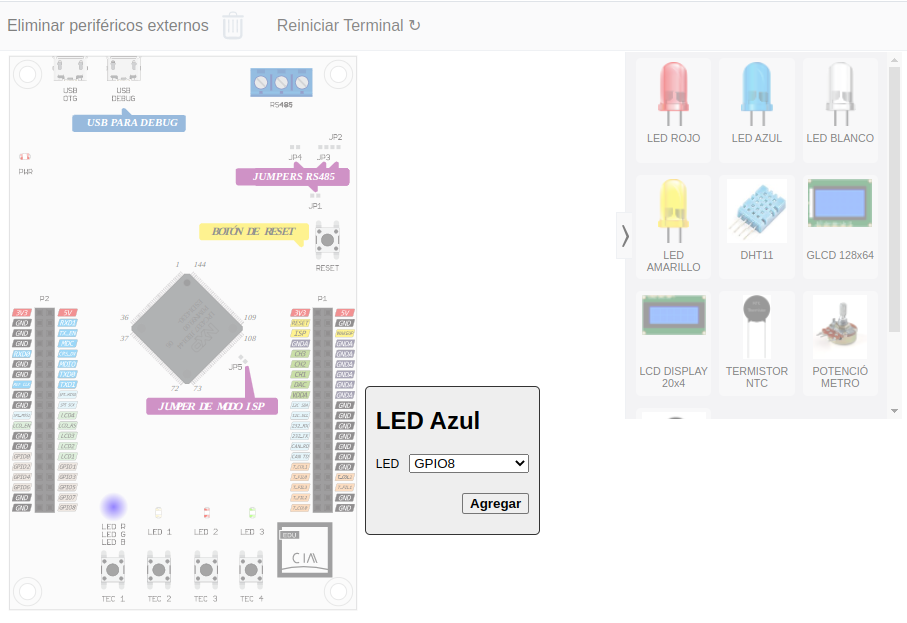
\includegraphics[scale=.45]{./Figures/AgregarPeriferico.png}
	\caption{Agregar periférico.}
	\label{fig:AgregarPeriferico}
\end{figure}


\begin{figure}[ht]
	\centering
	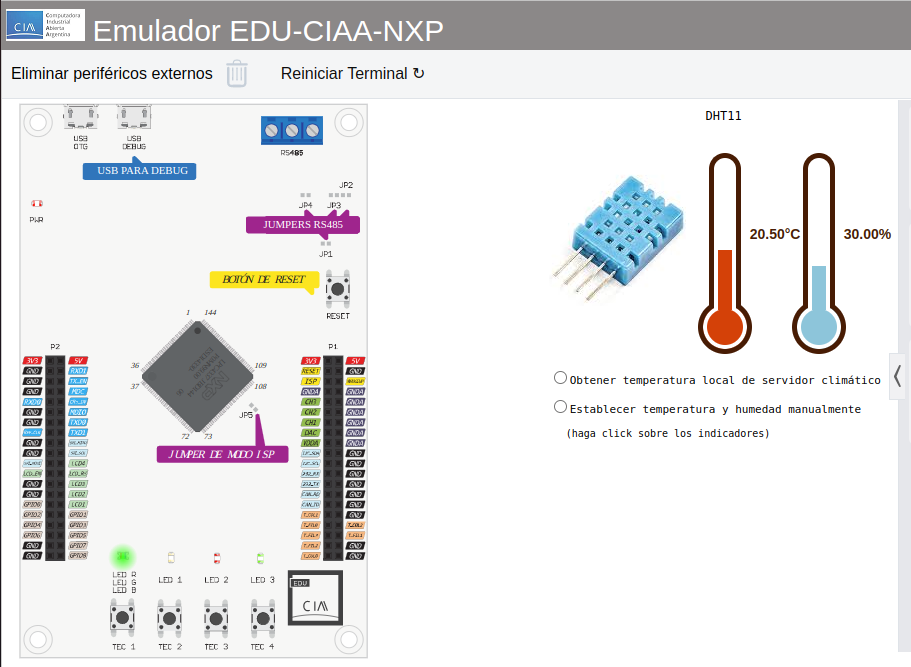
\includegraphics[scale=.45]{./Figures/AgregarPeriferico2.png}
	\caption{Periférico agregado en el área de ensamblado. }
	\label{fig:AgregarPeriferico2}
\end{figure}


\subsubsection{Área de codificación}

Esta parte de la plataforma se reserva al usuario para que pueda programar sus propias aplicaciones. Esta ventana de edición presenta las siguientes capacidades:

\begin{itemize}
\item Manejar la sintaxis para el lenguaje C.
\item Soportar el uso de las constantes, como por ejemplo: '\#define'.
\item Permitir el uso de las palabras claves, comentarios, etc.
\item Permitir el resaltado de líneas de código, sangría automática y número de línea.
\item Utilizar la función buscar (ctrl + f).
\item Utilizar la función buscar/reemplazar (ctrl + h).
\item Utilizar la función rehacer (ctrl + y).
\end{itemize}


Para compilar un programa, la plataforma provee al usuario el botón “ejecutar”. Sin embargo, si hubo problemas de sintaxis, errores lógicos, etc., se mostrarán esos errores al usuario.

En la figura \ref{fig:PlataformaErrores2} se muestra el código que generó los errores de compilación y en la figura \ref{fig:PlataformaErrores1} se observa los errores de compilación en el área de ensamblado.


\hfill \break
\hfill \break
\hfill \break
\hfill \break
\hfill \break
\hfill \break

\begin{figure}[ht]
	\centering
	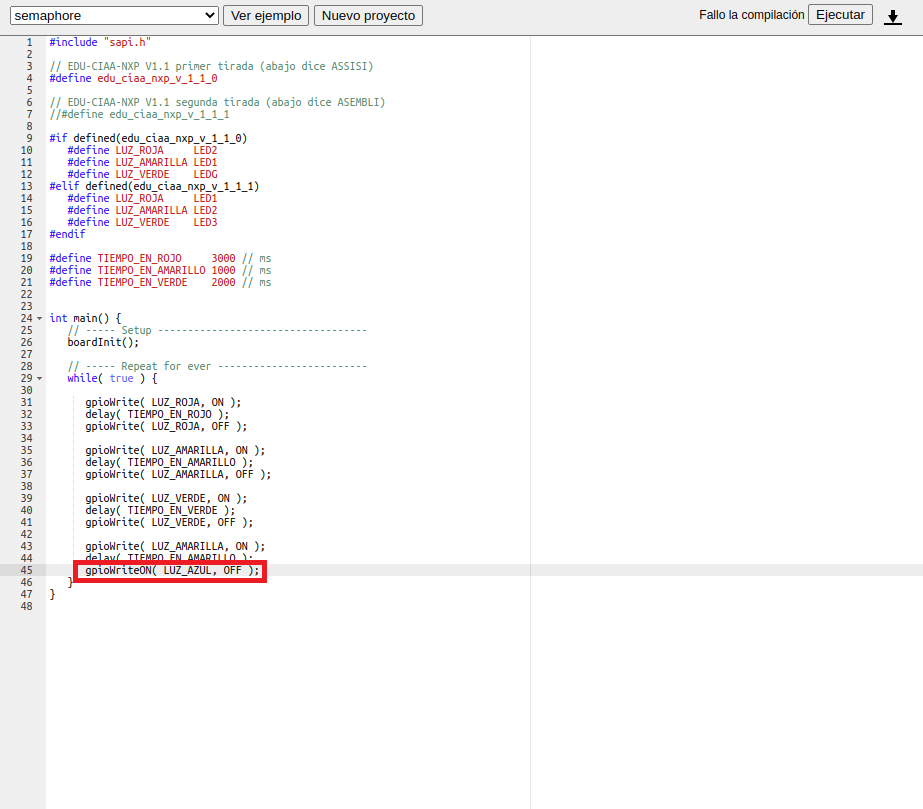
\includegraphics[scale=.40]{./Figures/PlataformaErrores1.png}
	\caption{Código que generó los errores de compilación.}
	\label{fig:PlataformaErrores2}
\end{figure}




\begin{figure}[ht]
	\centering
	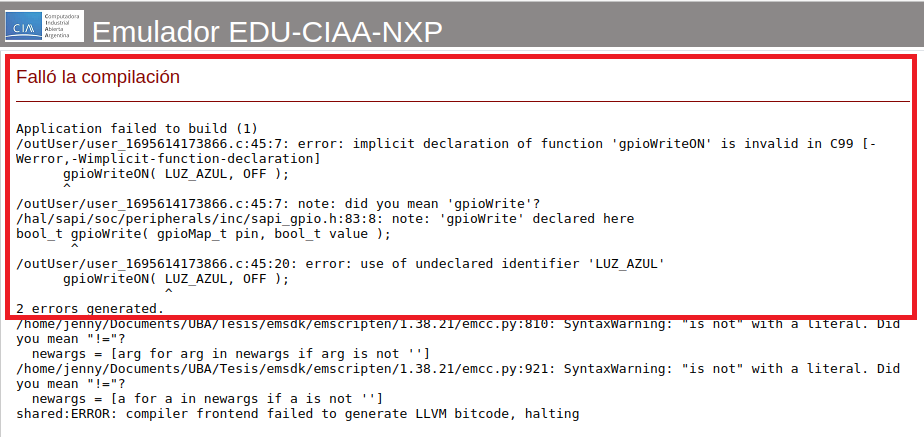
\includegraphics[scale=.40]{./Figures/PlataformaErrores2.png}
	\caption{Errores de compilación.}
	\label{fig:PlataformaErrores1}
\end{figure}

 
\subsubsection{Área de consola integrada}
Para el desarrollo de esta ventana se uso la biblioteca Xterm.js, que es un componente de terminal de front-end escrito en JavaScript y que permite construir terminales en el navegador. 

Entre las principales características se destaca:

\begin{itemize}
	\item Funciona con la mayoría de las aplicaciones de terminal, como bash, es compatible con aplicaciones basadas y eventos de mouse.
	\item Es de alto rendimiento, por eso es realmente rápido.
	\item No requiere de dependencias externas para funcionar, Sin embargo, la dependencia principal para el funcionamiento básico es el propio navegador web.
	\item API bien documentada.
\end{itemize}


Además de las características de Xterm.js, esta biblioteca de JavaScript es usado por varios proyectos populares como VS Code, Hyper y Theia que lo usan, de ahí que, el soporte en la comunidad de desarrolladores es amplio.

En la figura \ref{fig:Terminal1} se muestra un programa de usuario que generó la salida por consola.

\begin{figure}[ht]
	\centering
	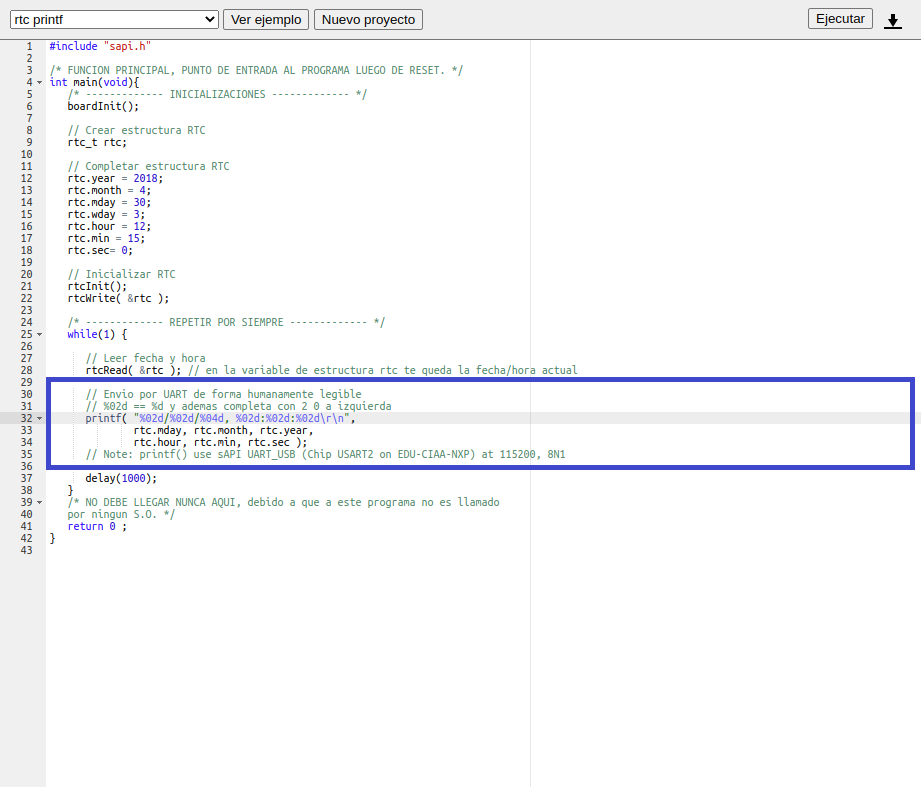
\includegraphics[scale=.41]{./Figures/Terminal1.png}
	\caption{Programa de usuario.}
	\label{fig:Terminal1}
\end{figure}
 


En la figura \ref{fig:Terminal2} se puede observar la salida por consola.

\begin{figure}[ht]
	\centering
	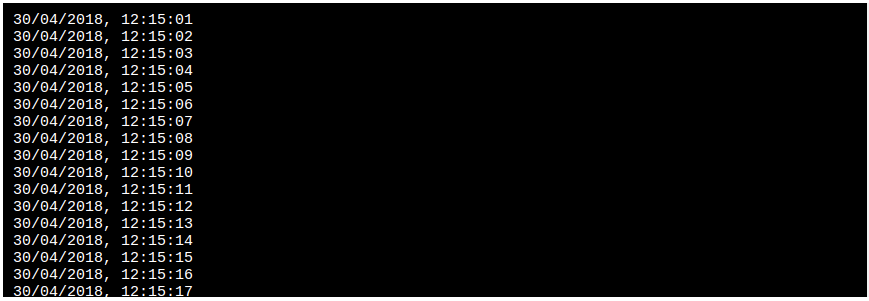
\includegraphics[scale=.45]{./Figures/Terminal2.png}
	\caption{Salida de la terminal serie.}
	\label{fig:Terminal2}
\end{figure}
 
 
Para ver el código del presente trabajo, se puede visitar el repositorio de GitHub \citep{repositorioEmulador}.


